\subsection{Имитационная модель. Схема эксперимента}

Для верификации развиваемых в работе подходов можно использовать данные, полученные при захвате в режиме онлайн или же
специально сгенерированные данные с использованием аппаратной или программной платформы. Преимуществом второго подхода
является то, что мы изначально знаем количество источников сигнала и их параметры (частоту, фазу ПСП, количество отраженных лучей).
В данной работе для верификации предложенных подходов будет использоваться второй пождход.

В разделе 1 уже рассматривались источники помех в системе с расширенным спектром Navstar GPS:
\begin{itemize}
	\item {данные эфемерид - ошибки в позициях спутников;}
	\item {часы спутника - ошибки в переданных данных о времени;}
	\item {ионосфера - ошибки в коррекции псевдодальностей обусловленных ионосферными эффектами;}
	\item {тропосфера - ошибки в коррекции псевдодальностей обусловленных обусловленных тропосферными эффектами;}
	\item {многолучевость - эффект отраженных сигналов принятых антенной;}
	\item {приемник - ошибки в измерениях обусловленные термальным шумом, точностью ПО и т.д.}
\end{itemize}

Генераторы сигнала можно разделить на программные и аппаратные. Программные генераторы позволяют сгенерировать
ВЧ сигнал с заранее заданными параметрами. В качестве аппаратных платформ для генерации сигнала можно использовать, например,
NI GPS Simulator. Данное решение позволяет сгенерировать практически произвольный сигнал за
счет большого количества настраиваемых параметров. Вместе с тем, аппаратные решения обладают существенным недостатком - высокая цена.

В данной работе будет использован программный подход к генерации сигнеала с расширенным спектром. В качестве модели была выбрана модель
сигнала с расширенным спектром СНС Navstar GPS. Существует много программных моделей данного сигнала,
например \cite{hannah_phd, burns_model, corbell_model, crs_model, brown_model}.

\subsection{Схема эксперимента}
Для проверки развиваемых в данной работе подходов построена имитационная модель системы передачи данных с ШПС.
Модель сигнала представлена в выражении \ref{eq:gps_signal}. Так как в работе развивается два подхода для сигнала
с АБГШ и с интерференционной помехой. Имитационная модель должна позволять выбрать необходимое количество источников сигнала.
Для проверки усовершенствованного алгоритма вычисления АКФ для компенсации окрашенной и белой аддитивной шумовой помехи
имитационная модель должна позволять добавлять АБГШ к генерируемому сигналу. 

Функциональная схема системы передачи информации представлена на рисунке \ref{pic:XXX}. Как уже было отмечено, бит данныx ${D_k(t)}$
принят за констату, так при ДФМ переход нарушает гармоническую структуру входного сигнала и детектирование становится невозможным,
она учтена в модели как неизвестная начальная фаза. Несущая сигнала модулируется заданной ПСП с периодом 1023 и длительностью 1 мкс.
Частота сигнала смещена на от центральной частоты для моделирования Допплеровского смещения. Рассолгасование и нестабильность
осцилляторов на стороне передатчика учтено в допплеровском смещении. Влияние этого рассогласования крайне невилико в сравнении
со смещением частоты, обусловленным допплеровским смещением в следствии движения передающего и принимающего сегментов.

К полученному сигналу добавляется ${K}$ дополнительных сигналов для создания интерференционной помехи от других источников,
так же добавляется АБГШ. Полученная смесь подавалась на алгоритм детектирования для определения рабочих характерстик развиваемых в работе подходов.

Модель сигнала может быть описана как:
\begin{center}
\begin{eqnarray}
	\label{eq:sec4_model}
	s_1(m)	& = & \cos(\omega_{1}m + \phi_1(m)) \nonumber \\
		& + & C_1(m) \sum \limits_{k=2}^{G}C_k(m)\cos(\omega_{k}m + \phi_k(m)) + n(m)
\end{eqnarray}
\end{center}где ${C_k(t)}$ - ПСП для ${k}$ - сигнала, ${\omega_{c}}$ - частота несущей сигнала, ${\phi_k(m)}$ - начальная фаза, равномерно распределенна ${[-\pi, \pi]}$
${G}$ - количество источников сигнала, ${n(m)}$ - АБГШ.

Количество источников сигнала ${G}$ задается с учетом распределения вероятностей количества источников для конктретной системы
связи с расширенным спектром. Для тестируемой системы Navstar GPS это распределение задается графиком (график приведен из стандарта Navstar GPS \cite{gpsuserequipment}):
\begin{figure}[ht]
	\center\scalebox{1}{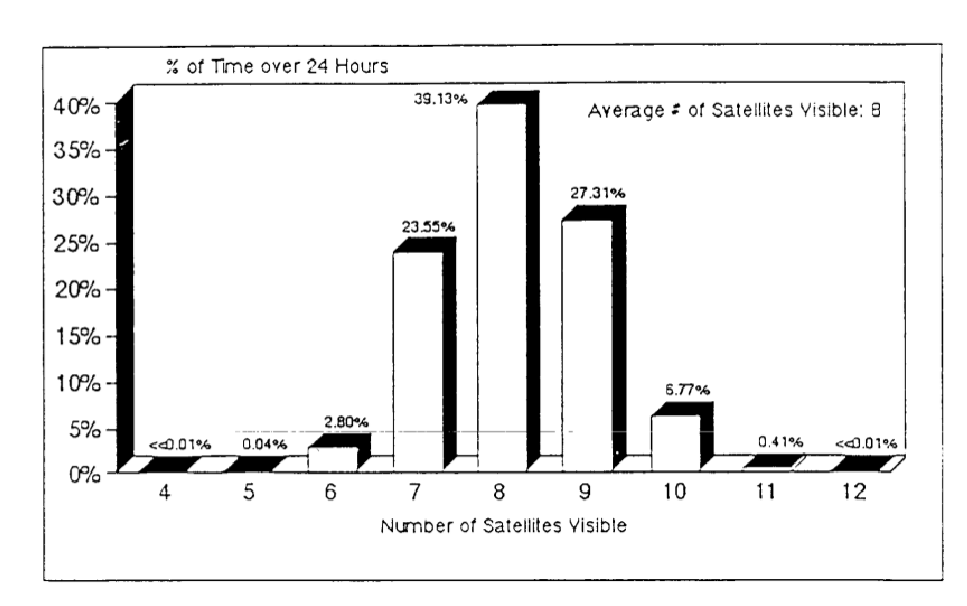
\includegraphics[width=1\linewidth]{gps_sats_num.eps}}
	\caption{Распределение количества источников сигнала}
	\label{pic:sec1_bpsk}
\end{figure}

\subsection{Экспериментальная проверка метода детектирования и оценки параметров сигнала при отсутствии интерференции на основе АР-модели}

Данный алгоритм рассмотрен в разделе \ref{l:sec3_lpc}. Особенностью данного алгоритма является является возможность детектирования сигнала
без перебора по частоте и позиции кода, в том смысле, в котором это понимается в параллельном корреляторе. Оценка частоты производится с
использованием АР-модели.

Таким образом для проверки предложенного алгоритма необходимо в имитационной модели задать один источник сигнала и задать уровень АБГШ для
тестирования рабочих характеристик предложенного алгоритма.

\subsection{Экспериментальная проверка метода детектирования и оценки параметров сигнала на основе АР-модели с использованием уточненной оценки АКФ
	и алгоритма Delay and Multiply Approach}

Данный алгоритм рассмотрен в разделе \ref{l:sec3_lpc_dma}. Данный алгоритм позволяет детектировать и оценивать параметры сигнала с расширенным спектром
на фоне АБГШ и интерференционной помехи. Таким образом для эффективной оценки алгоритма необходимо добавить ко входной смеси АБГШ и интерференционную помеху
для тестирования рабочих характеристик предлагаемого подхода.
